\chapter{Prehľad problematiky}\label{chap:issues_overview}

V tejto kapitole si popíšeme problémy, ktoré treba riešiť pri návrhu a implementácii GPS.
navigácie.
Problematiku tejto témy môžeme rozdeliť na dve logické časti a to problematika
GPS navigácie a problematika implementácie. Pri problematike GPS. navigácie
musíme brať do úvahy najmä funkčnosť GPS. navigácie, naopak pri problematike
implementácie sa budeme zaoberať výberom vhodných API a vhodným návrhom
architektúry samotnej aplikácie.

 

\begin{enumerate}
  \item Problematika GPS. Navigácie prostredníctvom webovej aplikácie
  \item Problematika implementácie
\end{enumerate}

\section{Problematika modelu peny}
  


\begin{itemize}
\item GPS
\item geolokácia
\item the w3c geolocation api
\item triangulacia
\item Google maps api
\item Kalmanov filter
\end{itemize}



\begin{itemize}
\item Úvod 
\item Klustrova analýza
\item Detekcia spôsobu presunu
\item Nájdenie cesty medzi dvoma bodmi
\end{itemize}  

\subsection{G.P.S.}

Global Positioning System, Globálny polohový systém, skrátene GPS, je vojenský družicový
navigačný prístroj prevádzkovaný Ministerstvom obrany Spojených štátov amerických, s ktorého pomocou je možné určiť geografickú polohu prijímača nachádzajúceho sa kdekoľvek
na Zemi alebo nad Zemou s presnosťou jednotiek metrov a tiež čas s presnosťou na jednotky
nanosekúnd. Presnosť určenia polohy s GPS je možné s použitím ďalších metód ešte zvýšiť
až na jednotky centimetrov. Časť služieb tohto systému s obmedzenou presnosťou je voľne k
dispozícii aj civilným používateľom.

\subsection{Primanie dát}

Užívatelia pomocou GPS prijímača prijímajú signály z jednotlivých družíc, ktoré sú v danú
chvíľu nad obzorom. Na základe prijatých dát (časových značiek z jednotlivých družíc a
znalosti ich polohy) a vopred definovaných parametrov prijímač vypočíta polohu antény
5
trianguláciou, nadmorskú výšku a zobrazí presný dátum a čas. Komunikácia prebieha iba od
družíc k užívateľovi, GPS prijímač je teda pasívny.


\subsection{Geolokácia}

Je metóda predpokladanie alebo identifikácia geografickej polohy objektu. Najbežnejšie
zahŕňa sadu geografických súradníc. Niektoré lokalizačne systémy často využívajú metódy
určovania polohy rádio frekvenciu. napríklad presnosť časového rozdielu príchodu (TDOA).
Systémy TDOA často používajú mapové zobrazenia alebo iný geografický informačný
systém. Ak nie je k dispozícii signál GPS, nealokačné aplikácie môžu použiť informácie z
bunkových veží alebo wifi na trianguláciu približnej polohy tuto metódu využíva w3c
geolocation api ktorú využíva naša aplikácia. 
 
\subsection{Triangulácia}

Triangulácia je proces, pomocou ktorého možno určiť polohu rádiového vysielača meraním
radiálnej vzdialenosti alebo smeru prijatého signálu z dvoch alebo troch rôznych bodov.
Triangulácia sa niekedy používa v bunkovej komunikácii na určenie geografickej polohy
používateľa.




\subsection{The W3C Geolocation API}

Je snahou o štandardizáciu rozhrania na získanie informácií o geografickej polohe pre
zariadenie na strane klienta.
v určitom časovom intervale nameraný bod obsahuje informácie o zemepisnej šírke , dĺžke,
výške, presnosti bodu a presnosti výšky, rýchlosti, smere pohybu. niektoré zariadenia
poskytujú iba súradnice a ich presnosť preto treba rýchlosť a smerovanie po poslednom
meraní dopočítať


\subsection{Funkčnosť}

Geolokátor obsahuje funkcie getcurrent position ,watchposition,showpozition
Get current a watch pozition služia na zistenie polohy.
Getcurrentpozition v časovom interval pošle informácie o poslednom meraní aj keď sa
nezmenila poloha naše riešenie využíva watchpozition na získanie nového merania
a showpoziton, ktorá zobrazí namerane hodnoty
Funkcia watchpozittition, ktorá v určitom časovom intervale nameria novú hodnotu ak sa
zmenila poloha zariadenia.
Nevýhody geolokátora: hlavnou nevýhodou je využitie wifi a mobilných sieti a chýbajúca
informácia o pôvode merania preto nevieme určiť odkiaľ boli namerane hodnoty. Nevyužitie
GPS senzora. Aplikácia zachytí najbližšiu wifi, ale prístupový bod. Preto namerané hodnoty
sú veľmi nepresné a počas merania by sa v polohe nedalo orientovať preto naša aplikácia
využíva kalmanov filter na vyhľadanie cesty a určenie skutočnej polohy zariadenia. Ďalšou
nevýhodou je nerovnomerné meranie v určitých časových intervaloch môžu vznikať zhluky
meraní. Preto pri filtrovaní v určitých prípadoch môže byť výsledná poloha iná ako naša
skutočná poloha 

\subsection{Google maps api }

Je webová mapovacia služba vyvinutá spoločnostou google. Ponuka snímky ulíc satelitné
síimky. Požíva sa na zobrazenie nameraných výsledkov na mape na spresnenie trasy dá sa
pomocou neho nájsť cesta medzi dvoma bodmi s využitím automobilu, pešou chôdzou,
s využitím hromadnej dopravy. Nevýhoda google maps - neaktuálne linky na zastávkach

\subsection{Kalmanov filter }

Tiež známy ako lineárny kvadraticky predpoklad je algoritmus ktorý používa sériu meraní
spozorovaných v čase obsahujúcich štatistiku hluku. Produkuje predpokladanú skutočnú
hodnotu ktorá je presnejšia ako naša nameraná hodnota.
Používa sa napríklad pri navigovaní.
Kalmanov filter používa dynamický model systému (napr. Fyzikálne zákony pohybu), známe
kontrolné vstupy pre tento systém a viacnásobné sekvenčné merania (ako napríklad zo
senzorov), aby vytvorili odhad merania(jeho stav, ktorý je lepší ako odhad získaný použitím
iba jedného merania samotného. Ako taký je spoločným algoritmom fúzie senzorov a dátovej
fúzie. Údaje o hlučných senzoroch, aproximácie v rovniciach, ktoré opisujú vývoj systému, a
vonkajšie faktory, ktoré nie sú zohľadnené pre všetky miesta, obmedzujú, ako je možné určiť
stav systému. Kalmanov filter účinne rieši odchýlku spôsobenú hlučným senzorom a do
určitej miery aj náhodnými vonkajšími faktormi. Kalmanov filter poskytuje odhad stavu
systému ako priemer predpovedaného stavu systému a nového merania pomocou váženého
priemeru. Účelom váh je, že hodnoty s lepšou (t.j. menšou) odhadnutou neistotou sú
"dôveryhodné" viac. Váhy sa počítajú z kovariancie, miery odhadovanej presnosti predikcie
stavu systému. Výsledkom váženého priemeru je nový odhad, ktorý leží medzi
predpokladaným a meraným stavom a má lepšiu odhadovanú presnosť ako samotne meranie.
Tento proces sa opakuje v každom časovom kroku, pričom nový odhad a jeho kovariantnosť
informujú predikciu použitú v nasledujúcej iterácii. Znamená to, že Kalmanov filter funguje
rekurzívne a vyžaduje iba posledný "najlepší odhad" skôr než celú históriu stavu systému na
výpočet nového stavu. Relatívna odchýlka meraní a odhadu súčasného stavu je dôležitým
aspektom a je obvyklé diskutovať o reakcii filtra v zmysle zisku Kalmanovho filtra. Zisk
Kalmana je relatívna váha daná meraniu a odhadu súčasného stavu a môže byť "naladená" na
dosiahnutie konkrétneho výkonu. S vysokým ziskom filter prikladá väčšiu váhu na najnovšie
merania, a preto ich viac zodpovedá. S nízkym ziskom filter sleduje predpovede modelu
užšie. V extrémnych situáciách dosiahne vysoký zisk blížiaci sa k jednej väčšej odhadovanej
trajektórii, zatiaľ čo nízky zisk blízko nuly vyrovná šum, ale znižuje citlivosť. Pri vykonávaní
skutočných výpočtov pre filter (ako je uvedené nižšie) sú stavové odhady a kovariancie
kódované do matíc na zvládnutie viacerých rozmerov zahrnutých do jednej sady výpočtov.
To umožňuje zobrazenie lineárnych vzťahov medzi rôznymi stavovými premennými
(napríklad pozícia, rýchlosť a zrýchlenie) v ktoromkoľvek z prechodových modelov.

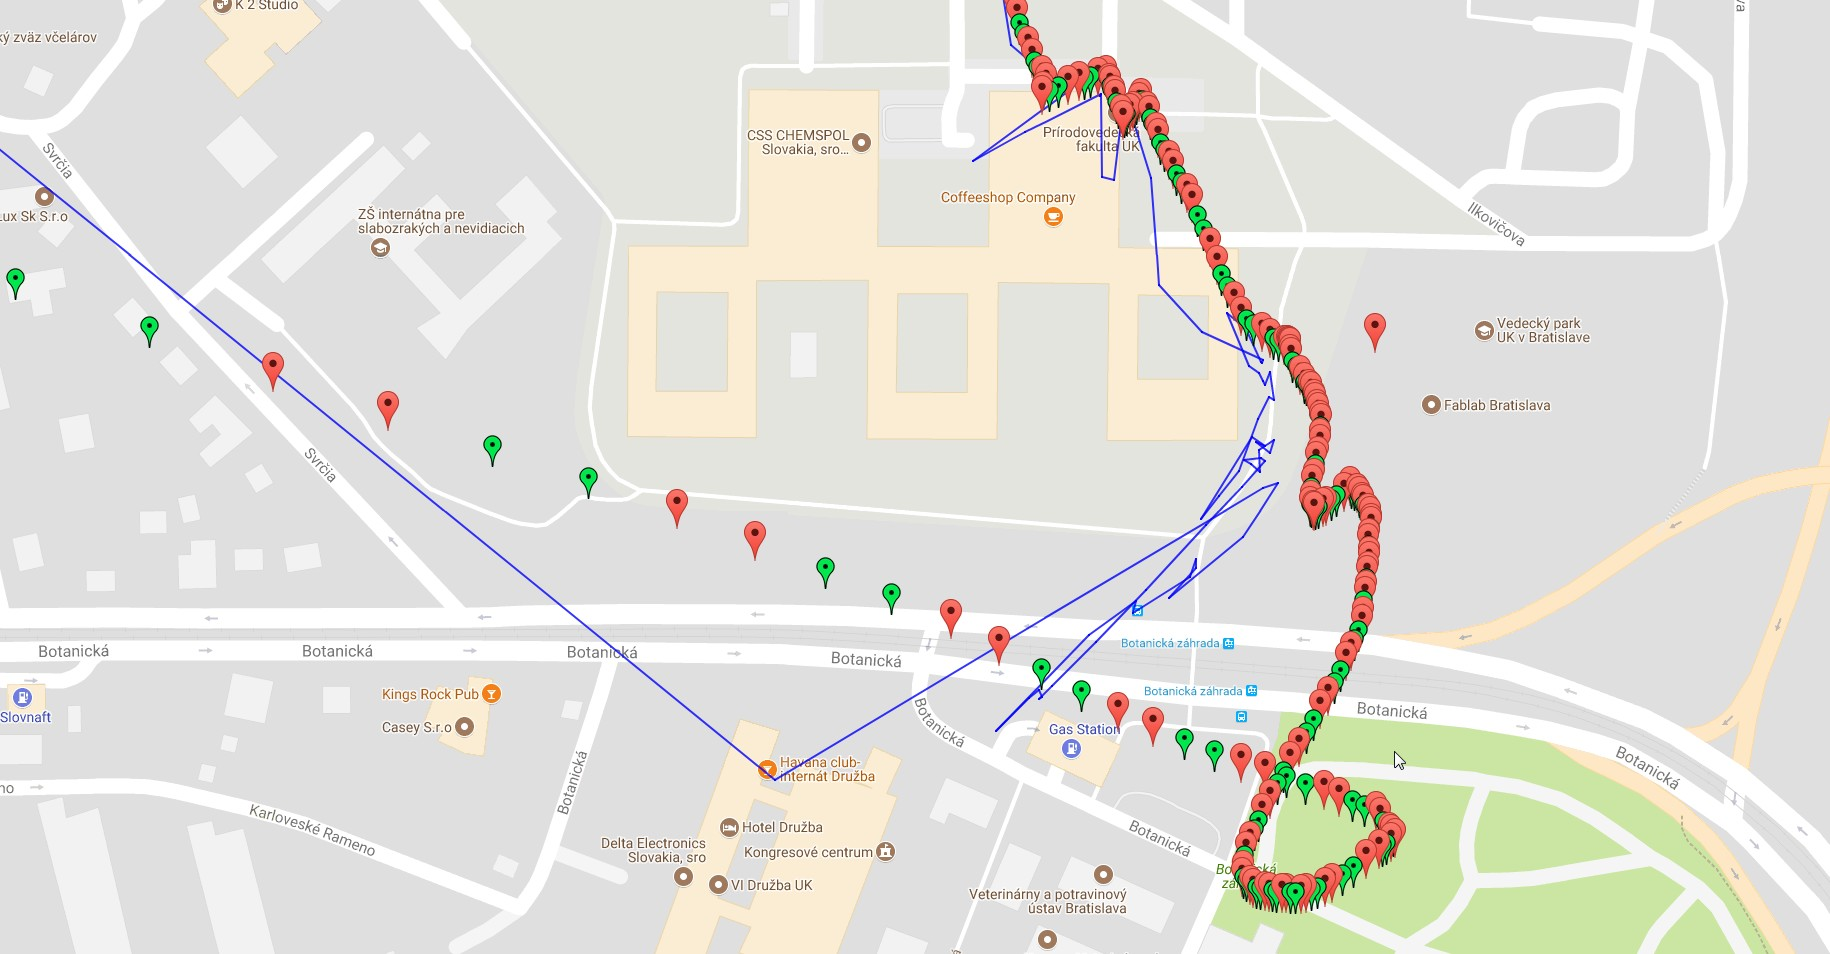
\includegraphics[width=\textwidth]{images/diplomka}
filtracia prejdenej nefiltrovanej cesty\\
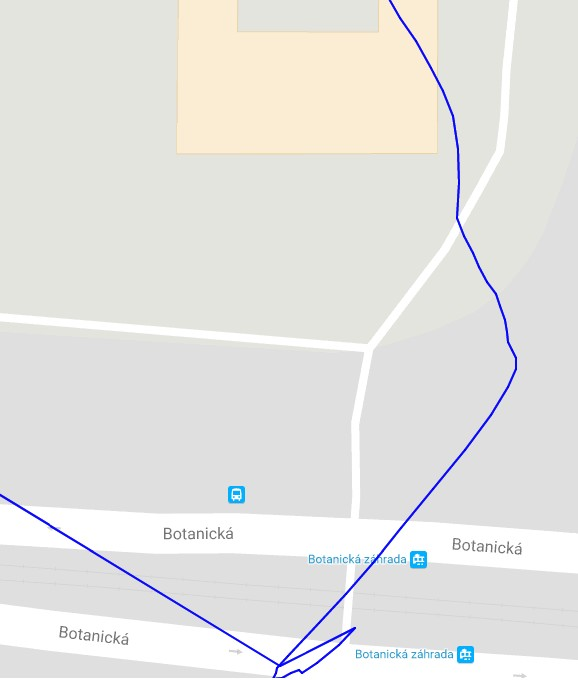
\includegraphics[width=\textwidth]{images/filtrovanie}
ta istá čaat cesty filtrovana počas presunu
\subsection{Google maps api }

Je webová mapovacia služba vyvinutá spoločnostou google. Ponuka snímky ulíc satelitné
síimky. Požíva sa na zobrazenie nameraných výsledkov na mape na spresnenie trasy dá sa
pomocou neho nájsť cesta medzi dvoma bodmi s využitím automobilu, pešou chôdzou,
s využitím hromadnej dopravy. Nevýhoda google maps - neaktuálne linky na zastávkach

\section{Problematika implementácie}

V predošlých podkapitolách sme popísali požite technológie pri takto zvolených metódach
dostaneme po ich aplikovaní filtra budeme mať presnejšie body, v tejto časti sa budeme
zaoberať problémami pri výpočtovej náročnosti geolokátora v reálnom čase. Pri tejto
problematike musíme riešiť:

\begin{itemize}
\item klustrová analýza
\item hľadanie cesty
\item výpočet rýchlosti 
\item detekcia spôsobu presunu
\end{itemize}

\subsection{klustrová analýza}

Zhluková analýza je zoskupenie množiny objektov takým spôsobom, že objekty v rovnakej
skupine (nazývané klastra) sú navzájom podobnejšie (v istom zmysle alebo inom) navzájom
než v iných skupinách (klastre) , Je to hlavná úloha prieskumného získavania údajov a bežnej
techniky analýzy štatistických údajov, ktorá sa používa v mnohých oblastiach vrátane
strojového učenia, rozpoznávania vzorov, analýzy obrazu, získavania informácií,
bioinformatiky,
Analýza klastrov sama osebe nie je jeden špecifický algoritmus, ale všeobecná úloha, ktorú
treba vyriešiť. To sa dá dosiahnuť rôznymi algoritmami, ktoré sa výrazne líšia v ich
predstavách o tom, čo predstavuje zhluk a ako ich efektívne nájsť. Medzi populárne pojmy
zhlukov patria skupiny s malými vzdialenosťami medzi členmi klastra, husté oblasti dátového
priestoru, intervaly alebo konkrétne štatistické rozdelenia. Zoskupovanie môže byť preto
formulované ako multi-objektívny optimalizačný problém. Príslušný klastrovací algoritmus a
nastavenie parametrov (vrátane hodnôt, ako je vzdialenosť, ktorú treba použiť, prahová
hustota alebo počet očakávaných klastrov) závisí od individuálneho súboru údajov a
zamýšľaného použitia výsledkov. Klastrová analýza ako taká nie je automatická úloha, ale
interakčný proces zisťovania poznatkov alebo interaktívnej viac-objektívnej optimalizácie,
ktorá zahŕňa skúšku a zlyhanie. Často je potrebné upravovať predbežné spracovanie údajov a
parametre modelu, až kým výsledok nedosiahne požadované vlastnosti.
Okrem pojmu clustering existuje niekoľko výrazov s podobným významom, vrátane
automatického triedenia, číselnej taxonomie, botryológie a
typologickej analýzy. Drobné rozdiely sú často v používaní výsledkov, zatiaľ čo pri získavaní
dát sú výsledné skupiny predmetom záujmu, v automatickom zatriedení je výsledná.
diskriminačná moc zaujímavá.
10
Základné členenie zhlukovacích metód podľa cieľa je na hierarchickej a nehierarchické
metódy.
Hierarchické zhlukovanie vytvára systém podmnožín, kde prienikom dvoch podmnožín -
zhlukov je buď prázdna množina, alebo jeden z nich. Pokiaľ nastane aspoň raz druhý prípad,
je systém hierarchický. Teda je to akési vetvenia, zjemňovanie klasifikácie. K hierarchickému
zhlukovaniu možno pristupovať z dvoch strán - rozlišujeme prístup divízny (vychádzame z
celku, jedného zhluku, a ten delíme) a aglomerativny (vychádzame z jednotlivých objektov,
zhlukov o jednom členovi, a tie spájame). Hierarchické zhlukovanie ponúka viac
alternatívnych riešení, výsledok zhlukovaniu je potom možné vyjadriť dendrogramem. Táto
metóda však nie je vhodná pre veľké dátové súbory.
Nehierarchické zhlukovaniu vytvára taký systém, kde sú zhluky disjunktné množiny. Používa
sa najčastejšie algoritmus k-means.
Zhluková analýza vychádza z podobnosti, respektive vzdialenosti objektov. Jej kvantitatívne
vyjadrenie je jedným zo základných problémov clusterové analýzy. Existuje mnoho spôsobov
konštrukcie tohto ukazovateľa.
Existujú rôzne prístupy, ako zhlukovať objekty na základe ich vzdialenosti alebo podobnosti.
Medzi základné metódy patria:
metóda najbližšieho suseda (single linkage, nearest neighbor) - vzdialenosť zhlukov je
určovaná vzdialenosťou dvoch najbližších objektov z rôznych zhlukov. Pri použití tejto
metódy sú objekty ťahané k sebe, výsledkom sú dlhé reťaze.
metóda najvzdialenejšieho suseda (complete linkage, furthest neighbor) - vzdialenosť
zhlukov je určovaná naopak vzdialenosťou dvoch najvzdialenejších objektov z rôznych
zhlukov. Funguje dobre predovšetkým v prípade, že objekty tvoria prirodzene oddelené
zhluky, nehodí sa, ak je tendencia k reťazeniu.
11
centroidná metóda - vzdialenosť zhlukov je určovaná vzdialenosťou ich centier (hypotetická
jednotka s priemernými hodnotami znakov). Môže byť nevážená alebo vážená. Tá
zohľadňuje veľkosti zhlukov a je vhodná ak očakávame ich rozdielnosť. Užíva sa vyjadrenie
vzdialenosti objektov štvorcovou Euclidean vzdialeností.
párová vzdialenosť (pair-group average) - vzdialenosť zhlukov je určovaná ako priemer
vzdialeností všetkých párov objektov z rôznych zhlukov. Opäť môže byť vo vážené i
nevážené podobe.
Wardová metóda - vychádza z analýzy rozptylu. Zlučuje také zhluky, kde je minimálna súčet
štvorcov. Všeobecne možno povedať, že je táto metóda veľmi účinná, však má tendenciu
vytvárať pomerne malé zhluky. Vzdialenosti objektov sa meria štvorcovou Euclidean
vzdialeností.
Hľadanie cesty medzi daným bodom bude riešené cez prehľadávanie na grafe

\subsection{Využitie clustra}

Aplikácia sa bude každý deň v určitom čase upravovať prejdené body v určitom rozmedzí sa
zhlukujú na jeden bod do tabuľky. Potom sa vytvorí cesta medzí dvoma bodmi, z ktorej sa pri
načítaní vytvorí graf


\subsection{Detekcia spôsobu presunu}

Aplikácia dostáva v určitých časových i intervaloch po nameraný sa nájde jeho skutočná
hodnota cez filter. Vypočíta sa vzdialenosť medzi poslednými bodmi, body od seba nemajú
veľkú vzdialenosť preto sa počíta z Pytagorovej vety potom sa vypočíta rýchlosť, ak je
rýchlosť väčšia ako 15 kilometrov predpokladaný presun je mestskou hromadnou dopravou


\subsection{Detekcia zastávok}

Aplikácia bude využívať presun hromadnou dopravou, da sa vyriešiť cez detekciu presunu,
za začiatok jazdy hromadnou dopravou by sme mohli označiť posledný bod s menšou
rýchlosťou. Označiť za zastávku, tu nastáva problém, autobus sa nepohybuje rovnakou 
13
rýchlosťou, preto nevieme určiť či autobus stoji v zápche, alebo na zastávke. Toto sa bude
riešiť na strane servera. 
za zástavku sa bude považovat bod z určitym počtom zastavení.


\subsection{Hľadanie cesty}

Pri zadaní cieľa a spustení sa nájde cesta do cieľa hľadaním cesty na grafe. Podľa zadaných
parametrov.
Parametre sú:
\begin{itemize}
	\item čas cesty
	\item vzdialenosť medzi začiatkom a koncom cesty
\end{itemize} cena cesty,\\


Pri zapnutí všetkých troch parametrov sa bude hľadať najlacnejšia cesta s najkratšou
prejdenou vzdialenosťou a najkratším časom.
Pri zapnutí parametra čas cesty a cena sa bude hľadať najlacnejšia cesta s najkratším časom.
Pri zapnutí parametra čas cesty a vzdialenosť sa bude hľadať najlacnejšia cesta z najkratšou
vzdialenosťou.
Ak nebudú používateľom zadane parametre bude sa hľadať najkratšia cesta.\\
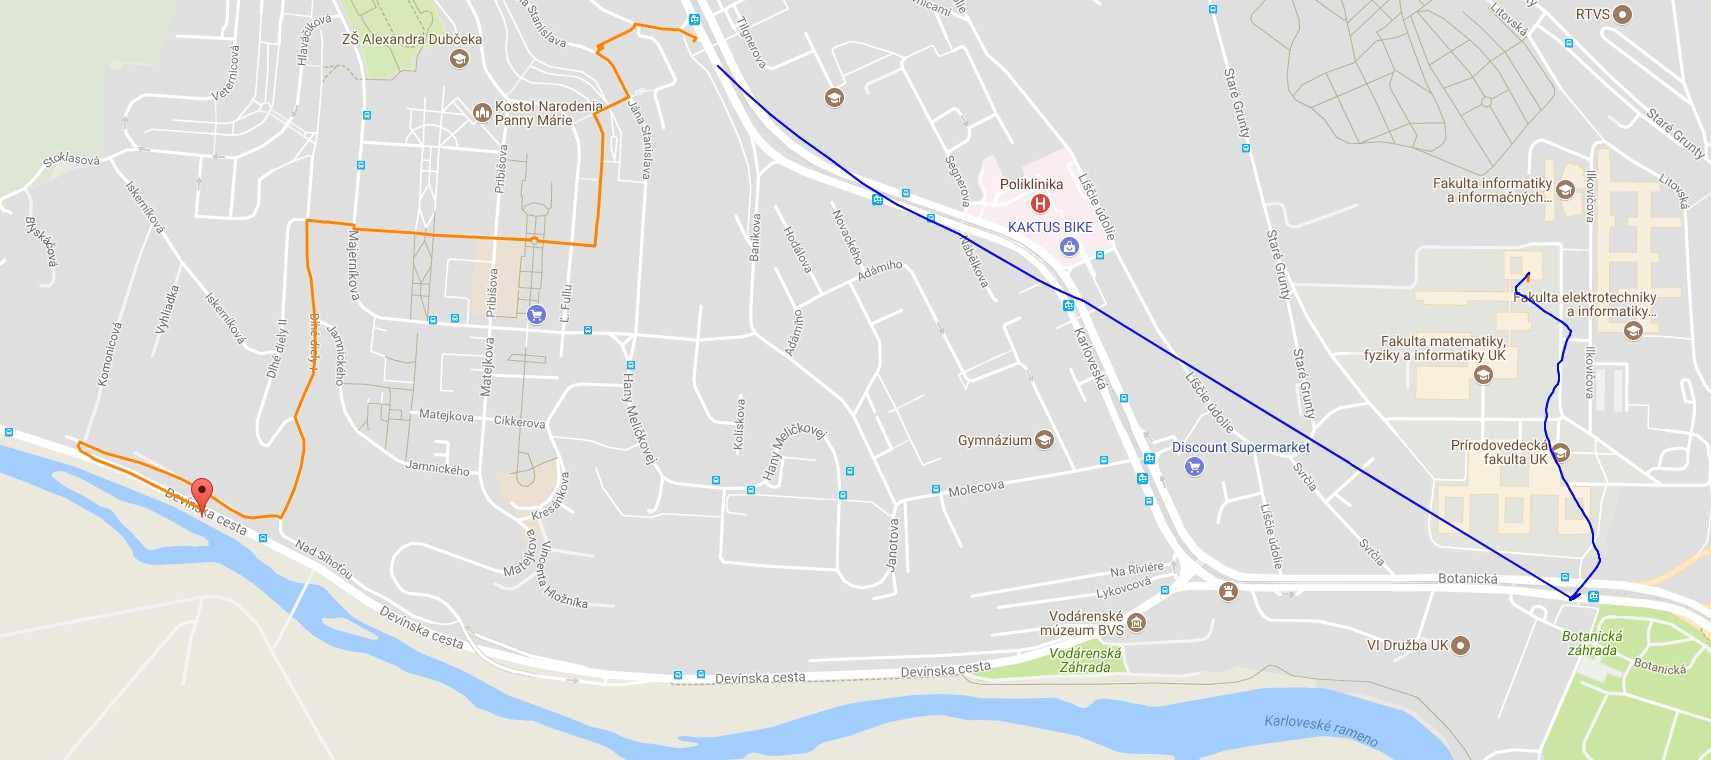
\includegraphics[width=\textwidth]{images/najdeniecesty}
nájdená cesta prehladavaním na grafe